\documentclass[11pt]{article}

\usepackage[utf8]{inputenc}
\usepackage{geometry}
\geometry{a4paper, margin=1in}
\usepackage{graphicx}
\usepackage{hyperref}
\usepackage{fancyhdr}

\setlength{\headheight}{15pt}
\pagestyle{fancy}
\fancyhf{}
\rhead{Computer Workshop Course}
\lhead{Final Assignment}
\rfoot{Page \thepage}

\title{Final Assignment}
\author{Mani Zamani}
\date{January 2025}

\begin{document}

\maketitle
\newpage
\tableofcontents
\newpage

\section{repository link}
\paragraph{\url{https://github.com/Manizmn84/FinalAssignment}}

\section{Git and GitHub}
\subsection{Repository Initialization and Commits}

\paragraph{To set up a repository, first of all, we must have a GitHub account. After creating a GitHub account or logging into the account, we perform the following steps:}

\begin{itemize}
    \item Go to the repository section in your account
    \item Click on New Repository
    \item Enter the explanation in the description field
    \item Choose whether the repository is public or private
    \item Choose "add README"
    \item Click on create repository 
\end{itemize}

\subsection{GitHub Actions for LaTeX Compilation}
\paragraph{Provide a walkthrough of setting up GitHub Actions to automatically compile your LaTeX document and any challenges you encountered.}
\paragraph{To launch a compiler for LaTeX with GitHub actions, you must set up a workflow and enter your codes for compilation in the `main.yml` file. It didn't work with tags on my system, so I had to go with push. One of the challenges I faced was that when I wanted to do it with tags, it wouldn't work, and I had to proceed with a push mode.}

\section{Exploration Tasks}
\subsection{Vim Advanced Features}
\paragraph{Explore and document 3 advanced features of Vim that were not covered in class:}

\begin{enumerate}
    \item One of Vim's features is macros, which allows you to record a sequence of keystrokes that can be executed with only one keystroke. This feature is useful for repetitive tasks, such as formatting code or generating boilerplate text.
    \item Another feature of Vim is the tabbed interface, which allows you to open many files and switch between them easily. This can be useful to save time when working with multiple files.
    \item The last feature is folding, which is useful for programmers and those working with large documents. It allows you to fold and unfold sections of text, making it easier to navigate and work with large files.
\end{enumerate}

\subsection{Memory profiling}
\subsubsection{Memory Leak}
\paragraph{\small A memory leak occurs when a programmer allocates memory but fails to free it.}

\subsubsection{Memory profilers}
\paragraph{\small Valgrind is an amazing tool used for identifying allocated memory. If you allocate memory and do not free it, Valgrind will detect it and provide information on allocated and freed memory, as well as the size of allocated memory.}

\subsection{GNU Linux Bash Scripting}
\subsubsection{fzf}
\paragraph{\small Fuzzy search is a search algorithm that allows users to ignore minor errors, such as misspellings, in one or a few letters of a word.}
\paragraph{\small To install `fzf` and understand the command: \texttt{ls | fzf}, this command helps you navigate and select files or directories using fuzzy search. The `ls` command lists the files, and with `fzf`, you can quickly search through them.}

\subsubsection{Using fzf to find your favorite PDF}
\paragraph{\small To find a specific PDF file quickly, install `fd` and run \texttt{fd -e pdf} to list all PDF files in a directory. You can refine the search with \texttt{fd -t -e pdf} to search within subdirectories as well. To select a specific file, use \texttt{fd -t pdf -E '.*' file name | fzf}.}

\subsubsection{Opening the file using Zathura}
\paragraph{\small To open the selected file in Zathura, use the command: \texttt{fd -t pdf -E '.*' | fzf \&\& zathura (\$cat -)}. The \texttt{cat -} command passes stdin to Zathura, allowing it to open and display the selected file.}

\section{Git and FOSS}
\subsection{README.md}
\paragraph{write in README.md file}

\subsection{Issues}
\begin{figure}[h]
    \centering
    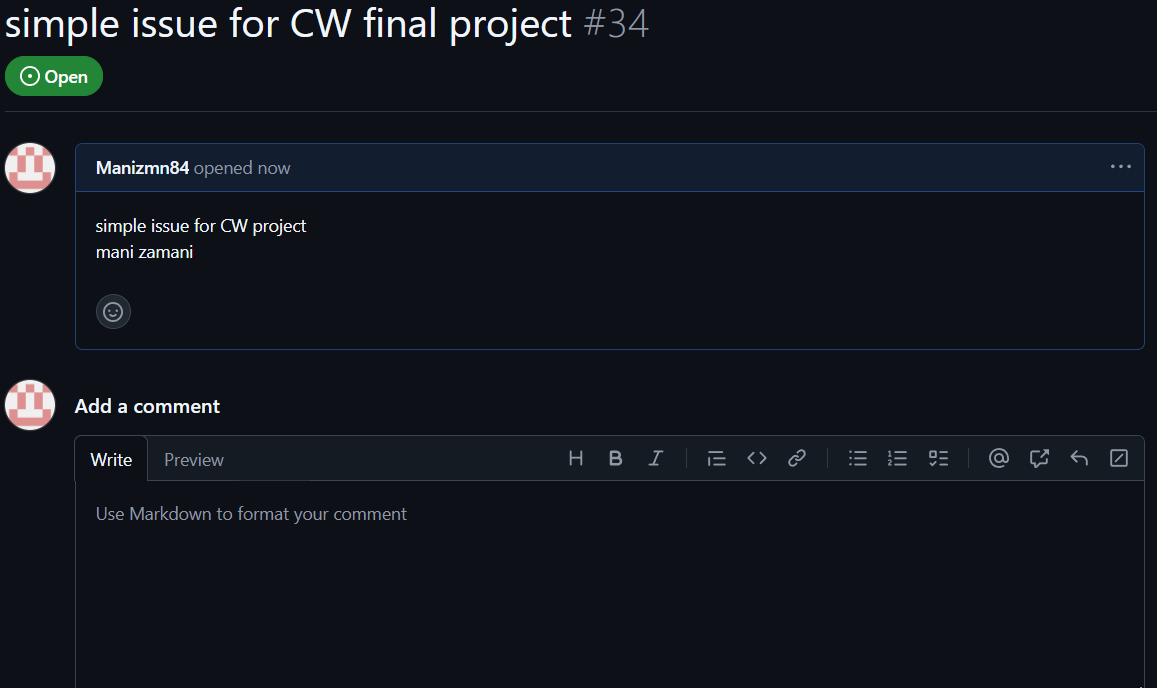
\includegraphics[width=0.5\textwidth]{issue.png}
    \caption{simple issue}
\end{figure}    


\end{document}